\begin{frame}{Redefine the problem} 
    \centering
    \textbf{Can we design an omni-directional wheeled robot \\
    to meet these requirements?}
\end{frame}

% \begin{frame}{Solution}
    
% \end{frame}

\begin{frame}{Reference} 
\footnotesize{
\begin{thebibliography}{99}
[1] W. Reid, F. J. Pérez-Grau, A. H. Göktoğan and S. Sukkarieh, Actively articulated suspension for a wheel-on-leg rover operating on a Martian analog surface, 2016 IEEE International Conference on Robotics and Automation (ICRA), 2016.
\end{thebibliography}

\begin{thebibliography}{99}
[2] Y. Xu, J. Tu, G. Tang, Robust navigation control of a 4WD/4WS agricultural robotic vehicle, Computers and Electronics in Agriculture, Volume 164, 2019.
\end{thebibliography}

\begin{thebibliography}{99}
[3] M. Bjelonic et al., "Keep Rollin’—Whole-Body Motion Control and Planning for Wheeled Quadrupedal Robots," in IEEE Robotics and Automation Letters, vol. 4, no. 2, pp. 2116-2123, April 2019.
\end{thebibliography}
}

\end{frame}

\begin{frame}{End} 
    \centering
    \textbf{Thanks For Your Listening! \\ Q\&A}
\end{frame}




% \begin{frame}{Solution} 
% \begin{columns}
% \column{0.5\textwidth}
    
% \column{0.5\textwidth}
% \begin{figure}
%     \centering
%     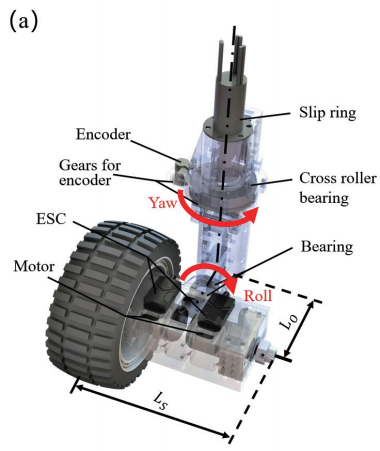
\includegraphics[width=4cm]{photos/ASOC_module.png} 
%     \vspace{-0.3cm}
%     \caption{ASOC module}
%     \label{fig:mine}
%     \vspace{-0.7cm}
% \end{figure}
% \end{columns}
% \end{frame}